\chapter{Velká data v~Průmyslu 4.0}\label{kap:industry4.0}
Vize Průmyslu 4.0 spočívá v dokončení digitalizace a automatizace průmyslu a směřování k~autonomním továrnám. Dochází k~propojení počítačových systémů zavedených v~předchozí fázi třetí průmyslové revoluce a také všech součástí výrobního procesu včetně strojů. Právě průmyslové stroje jsou potenciálním zdrojem obrovského množství užitečných informací. U~strojů lze sledovat například kvalitu výstupních produktů, vibrace či teplotu jednotlivých částí. Tyto informace umožňují rychlou detekci a předpověď poruch v~reálném čase nebo zaznamenávání vytížení stroje v~konkrétních fázích výroby. Agregovaná data mohou posloužit k~vyhodnocení výrobních procesů, nalezení slabých míst a následnému zefektivnění jednotlivých procesů. 

V~poslední době jsou nasazovány takzvané chytré stroje, osazené různými senzory a výpočetními jednotkami pro sběr dat a komunikaci se zbytkem systému. Nejen nové stroje nabízí možnosti propojení s~celým systémem, mnoho firem se zaměřuje na osazování starých strojů senzory a výpočetními jednotkami, aby i tyto stroje mohly být monitorovány a propojeny se systémem. Příklady těchto firem a jejich produktů jsou popsány dále v~této kapitole.


%popsat průmysl 4.0 TODO
%https://www.systemonline.cz/rizeni-vyroby/uvod-do-problematiky-a-zakladni-modely-industry-4.0.htm
%https://www.forbes.com/sites/bernardmarr/2018/09/02/what-is-industry-4-0-heres-a-super-easy-explanation-for-anyone/#3f2f13779788
%https://link.springer.com/chapter/10.1007/978-3-030-14544-6_4
%https://www.researchgate.net/publication/315472746_Big_Data_for_Industry_40_A_Conceptual_Framework
%https://www.datanami.com/2019/04/25/big-data-challenges-of-industry-4-0/
%https://controlstation.com/what-are-the-differences-between-industry-4-0-big-data-and-the-iiot/


\section{Využití velkých dat v~průmyslu}
Faktické informace k využití velkých dat byly čerpány z \cite{bigDataUse}. Velká data mají v~dnešním průmyslu široké využití ve všech odvětvích. V~chemickém odvětví se využívají k~analýze vnějších vlivů, jako teploty či tlaku, na výsledný produkt. Umožňuje tak úpravu těchto vlivů, což přináší až pětinové snížení produkce odpadních látek či šestinovou úsporu energie. Stejným způsobem dochází ke zkoumání vlivu různých faktorů na produkci i v~průmyslu farmaceutickém, kde dochází až k~padesátiprocentnímu navýšení produkce díky analýze velkých dat. Další odvětví, kterému analýza velkých dat pomáhá, je automobilový průmysl. Data získaná a zpracovaná z~prototypů či již produkčních vozidel umožňují rychlé zjištění slabin či chyb ať už návrhové či produkční fázi vozidel. Následně je možné v~produkci tyto chyby rychleji odstranit a tím docílit menších nákladů při dodatečných opravách. Další využití nachází energetický průmysl. Například u~větrných elektráren se již dnes využívá analýza velkého množství dat ze senzorů pro ovládání větrných turbín a maximalizaci efektivity při výrobě energie. Historická data a data získávaná v~reálném čase následně slouží k~vytváření prediktivních modelů pro optimalizaci provozu nejen elektráren a pro ulehčení rozhodování vrcholového managementu a to ve všech průmyslových odvětvích. 


\section{Existující systémy}
Jak již bylo zmíněno, Průmysl 4.0 je velmi rychle se rozvíjející obor. Stejně rychle vznikají systémy pro sběr a zpracování velkých dat pro průmysl. Jednou z~vlastností průmyslu je jeho rozmanitost. Tím je myšleno obrovské množství specializovaných strojů a postupů, které se používají v~jednotlivých odvětvích. Tato variabilita způsobuje to, že je velice těžké, a nákladné vytvořit univerzální systém. Právě z~toho důvodu je velká část jak hardwarových, tak i softwarových řešení, specializovaných. Zároveň existuje nepřeberné množství parametrů, které lze sledovat -- od teploty vzduchu v~provozu až po výkonnost zaměstnanců. Tato sekce se zabývá existujícími hardwarovými a softwarovými řešeními pro sledování stavu průmyslových strojů (teploty, vibrací, otáček a podobně).

%\subsection{Apache Hadoop}\label{apache-hadoop}
%Apache Hadoop je volně dostupný framework, umožňující distribuované zpracování velkého množství dat %napříč větším množstvím výpočetních uzlů. 

\subsection{Hardwarové řešení}
Zařízení pro sběr velkých dat se dají rozdělit na jednoúčelová a víceúčelová. Jednou ze zahraničních firem věnujících se vývoji jednotek pro sběr a zpracování dat je National Instruments. Firma se zabývá vývojem automatizovaného testovacího vybavení a nabízí celý ekosystém výrobků, mimo jiné i pro sběr dat ze senzorů a zpracování signálu. Pro sběr a zpracování dat nabízí jednotku cRIO zobrazenou na obrázku \ref{pic:rio}. Toto zařízení je víceúčelové. Velkou výhodou je, že zařízení obsahuje kromě procesoru i programovatelné hradlové pole neboli FPGA, umožňující optimalizovat některé výpočty přímo na jednotce. Další výhodou je možnost připojení velkého množství rozšiřujících modulů pro různé vstupy, od bezpečnostních modulů přes zvukové moduly až po drivery motorů. Velkou nevýhodou je cena. Plně vybavené zařízení s~potřebnými rozšiřujícími moduly a softwarem pro programování může vyjít na statisíce korun za kus \cite{rio}.

Příkladem jednoúčelových zařízení může být jednotka partnerské firmy zvaná Chipmunk. Jednotka je zobrazena na obrázku \ref{pic:4dotchip}. Zařízení obsahuje pouze procesor bez hradlového pole a není rozšiřitelné o~moduly. Zařízení má pevně dané čtyři vstupy pro senzory vibrací se snímáním o~vzorkovací frekvenci až 128 kHz \cite{4dotchipmunk}. Kromě této firmy existují nejen ve světě, ale i v~České republice, desítky firem vyvíjející podobné jednotky, určené ke sledování nepřeberného množství různých parametrů strojů. Jednoúčelové jednotky sice nabízí oproti víceúčelovým mnohem užší spektrum využití, zato jsou dostupné za řádově nižší cenu a jsou vhodnější pro masové nasazení.

\begin{figure}[h]
  \centering
  \begin{minipage}[b]{0.45\textwidth}
    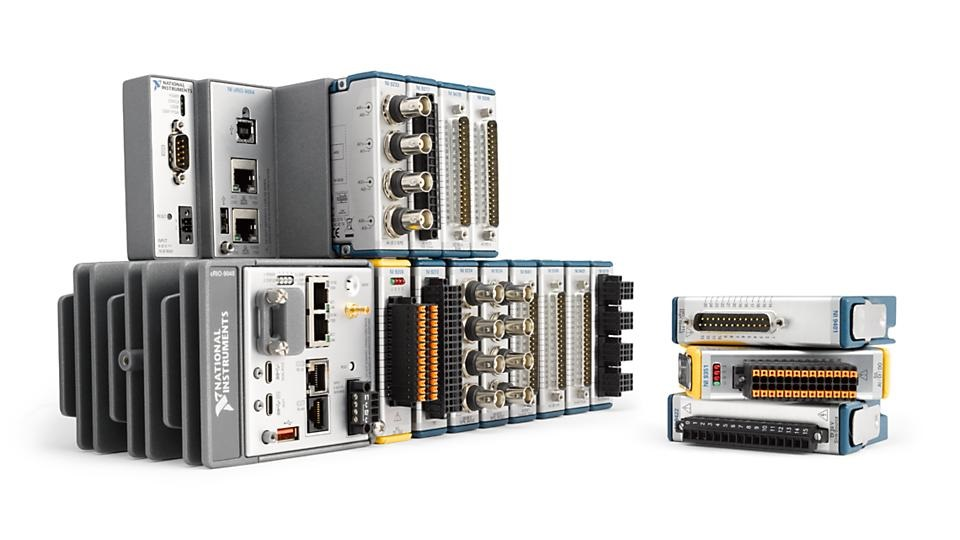
\includegraphics[width=\textwidth]{obrazky-figures/rio.jpg}
    \caption{Jednotka cRIO s~rozšiřujícími moduly \cite{rio}.}
    \label{pic:rio}
  \end{minipage}
  \hfill
  \begin{minipage}[b]{0.45\textwidth}
    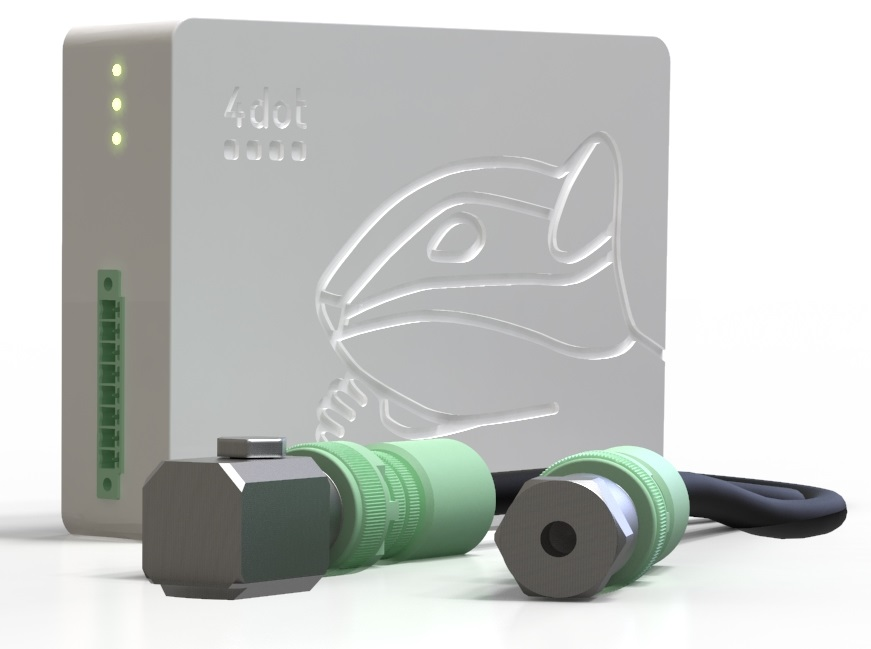
\includegraphics[width=\textwidth]{obrazky-figures/chipmunk.jpg}
    \caption{Jednotka Chipmunk se senzory vibrací \cite{4dotchipmunk}.}
    \label{pic:4dotchip}
  \end{minipage}
\end{figure}


\subsection{Softwarové řešení}
Softwarové řešení pro sběr a zpracování dat má dvě základní části. První částí je softwarové vybavení, kterým jsou vybaveny jednotky. Ty data sbírají, a v~omezené míře i zpracovávají. Druhou částí řešení jsou centralizované serverové aplikace sbírající a zpracovávající data od jednotek. Tyto aplikace se starají také o~přístup k~výsledným informacím a jejich vyhodnocení. 
Existují i lokální řešení, která jsou omezena pouze na jednotku poskytující informace přímo u~monitorovaného stroje (například na monitor). Tyto jednotky dále nekomunikují s~jinými zařízeními. Takovým systémům se však tato podsekce nevěnuje, protože nesplňují cíl Průmyslu 4.0 -- úplné propojení všech částí do jednoho celku.

Software obsažený v~jednotkách je často vytvořen přímo firmou, která vyvinula dané zařízení. Se systémem komunikuje pomocí řady standardizovaných protokolů určených pro průmysl. Příkladem může být jednotka pro monitorování vibrací společnosti ifm\footnote{https://www.ifm.com/gb/en/category/070/070\_010/070\_010\_015\#!/S/BD/DM/1/D/0/F/0/T/24} s~možností výběru komunikačního rozhraní jako je PROFINET IO, Modbus, EtherCAT. Jinou cestou se vydala již zmíněná americká společnost National Instruments, která prodává jednotky bez softwarového vybavení. Programy pro tyto jednotky se vytváří v~programu zvaném LabView\footnote{https://www.ni.com/cs-cz/shop/labview.html} a opět lze volit různá komunikační rozhraní. Více informací ke komunikačním protokolům je obsaženo v~sekci \ref{sec:networkComm}.

\begin{figure}[h]
  \centering
  \scalebox{0.29}{
        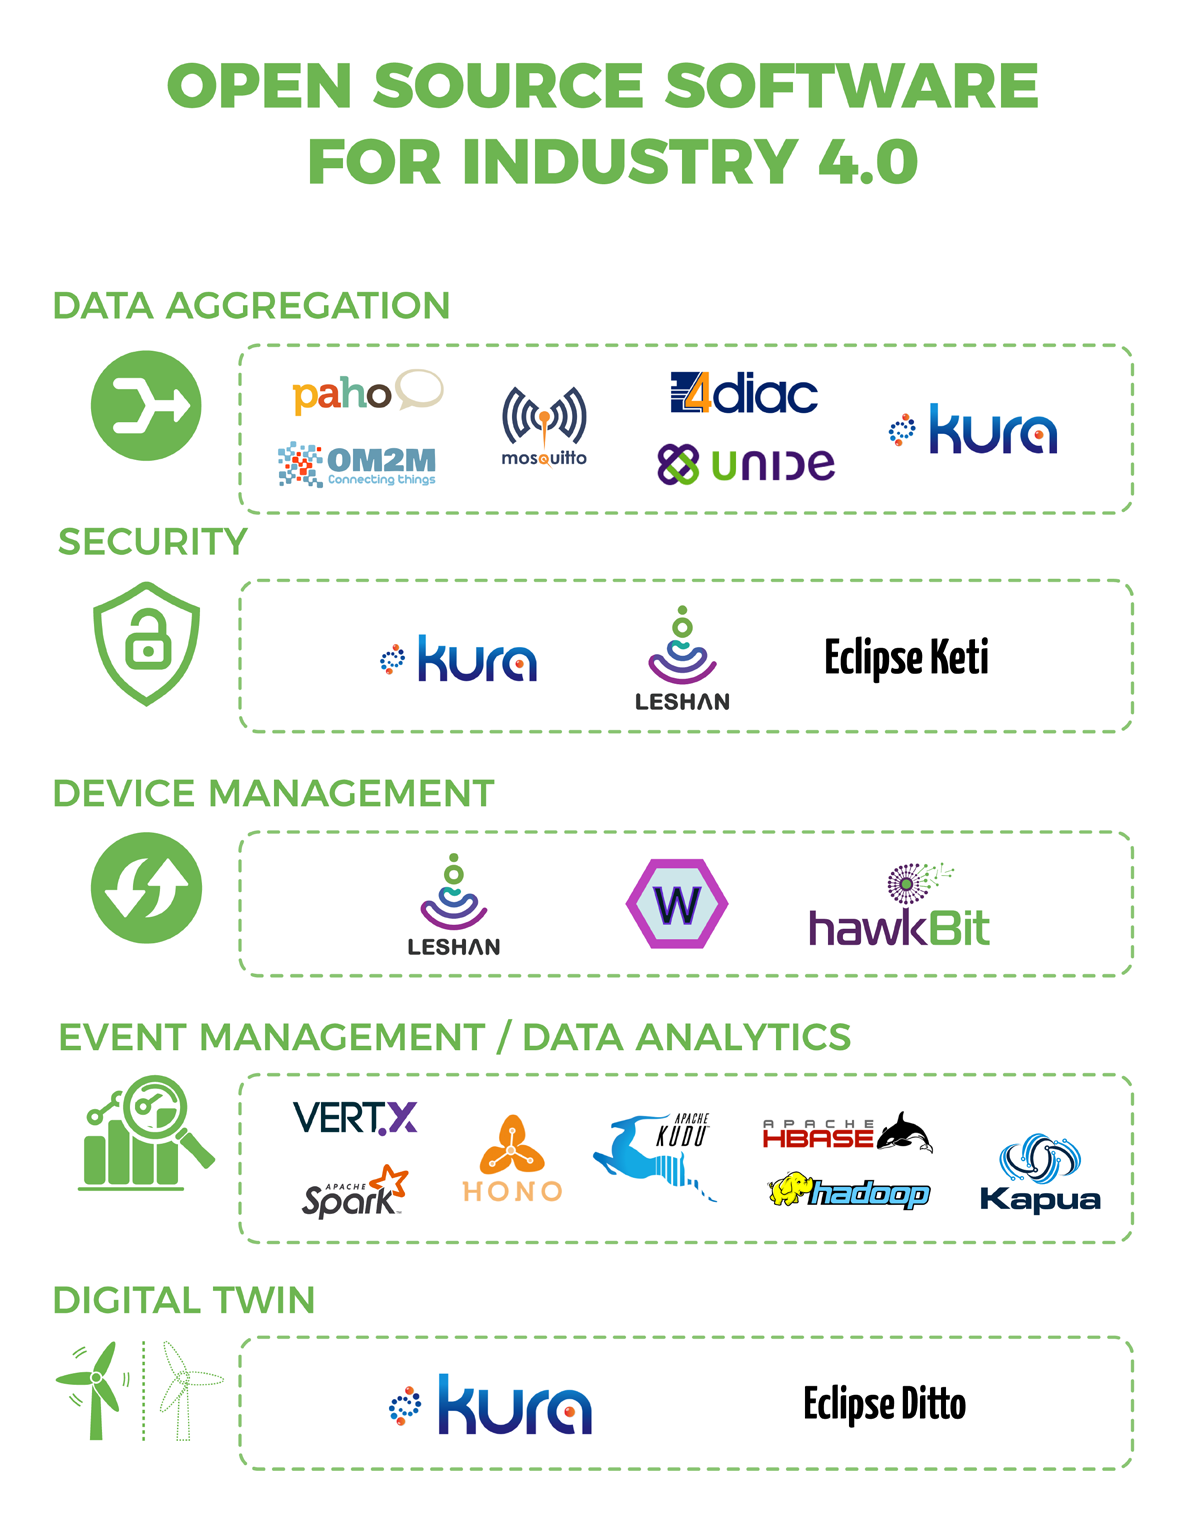
\includegraphics{obrazky-figures/open_source_iot.png}
    }
  \caption{Kategorie komponent systému pro Průmysl 4.0 a jejich zástupci \cite{eclipse}.}\label{pic:eclipseIOT}
\end{figure}

Serverová část systému slouží k~příjmu dat od jednotek, jejich zpracování a uložení. Tyto systémy mohou mít mnoho funkcí a řadu různých komponent. Komponenty se mohou dělit podle funkce do několika kategorií: příjem dat a agregace, zabezpečení, správa zařízení, správa událostí, datové analýzy, datová úložiště a další. Existuje velké množství implementací jednotlivých komponent a to nejen placené, ale i volně dostupné pod open-source licencemi. Příklady zástupců jednotlivých kategorií jsou zobrazeni na obrázku \ref{pic:eclipseIOT}.

Implementaci některých komponent nabízí společnost Eclipse. Příkladem může Eclipse Paho a Eclipse Mosquitto implementující protokol MQTT  (Message Queuing Telemetry Transport). Velká sada softwarových komponent vhodných pro Průmysl 4.0 spadá pod Apache Software Foundation, která obsahuje mimo jiné i nástroje pro distribuované zpracování dat a výpočty či distribuovaná úložiště \cite{eclipse}.

Serverové řešení jako takové tedy není omezeno na jednu určitou implementaci jako u~jednotek, ale je možné vybírat z~různých volně dostupných či placených komponent a postavit systém na míru podle potřeby a využití.

%Například Apache Hadoop je nástroj sloužící pro distribuci zpracovávání velkého množství dat na více výpočetních uzlů s důrazem na snadnou škálovatelnost



